\chapter{Research Methodology}
\label{ch:researchmethodology_report}

\section{User Experience Design} 
\label{sec:uxd}

User Experience (UX) Design plays a vital role in the success of a product but often underestimated. In a typical software industry, they say reasons to like it might lead to over budget or no time to skip it and get right into the development phase. Well, a User Experience Design process is far beyond what we know as User Interface Design or Usability. Wireframe tool is typically used to design user interface, and usability is a way of testing whether the designed product is usable enough. A User Experience (UX) Design is a user-centred process which emphasis on the context of the user and his needs rather than focusing solely on interface design. \cite{UX} For example, let us say someone designed a navigation application where the user says that he wants to reach from location A to location B, and it displays the route. Now, what if the user wants to mention points as a market name instead of street name and when underlying database consists only street names, that is a bad user experience (UX) even though the application is designed with better UI and also usable? Its Design \cite{UXD} cycle, as seen in the \autoref{fig:ux-design} illustrates an iterative cycle where we gather requirements. Next, we make a prototype based on the requirements and then test the designs with assumed metrics which serve as quantitative feedback and reasonings serve as qualitative feedback. Then based on the user feedback, we gather new requirements for next cycle. The iterations continue as long as we have betterment in the usability of designs proposed which enhances the user experience. \\ \\


\begin{figure}[hbt!]
	\centering
	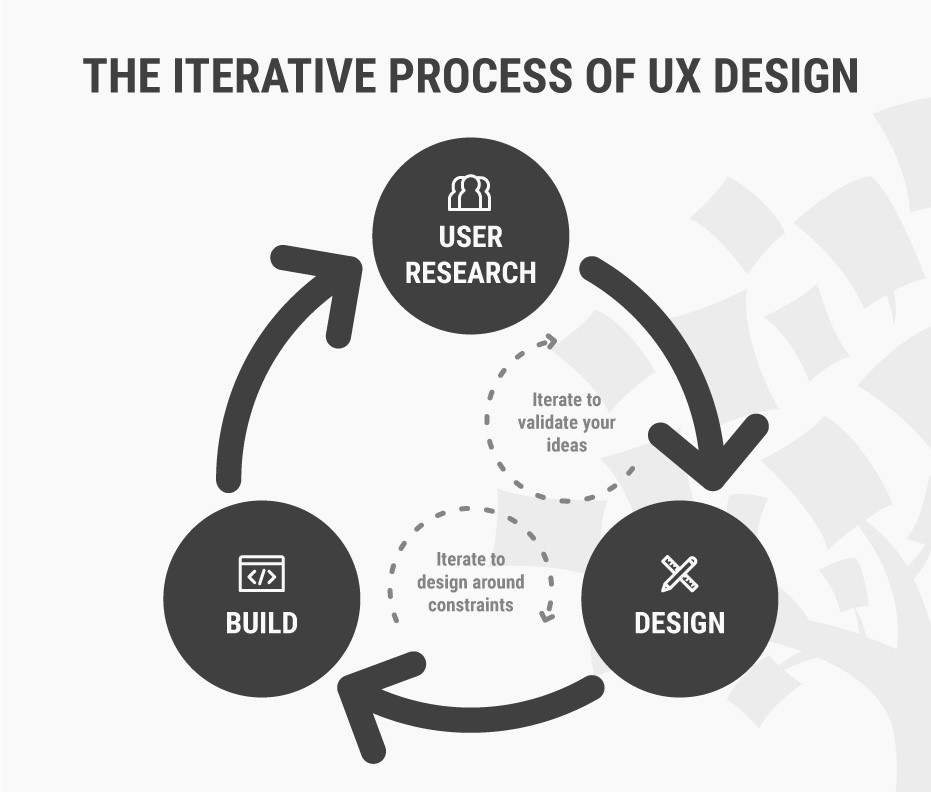
\includegraphics[width=\linewidth]{figures/ux-design}
	\caption{UX-Design.\cite{UXD}}
	\label{fig:ux-design}
\end{figure}

We can see the applicability of the User Experience Design in detail at Chapter \ref{ch:approaches_report}. \\ \\


\section{Evaluation Process}

We test the prototypes mentioned in the later chapters as per the experimental design guidelines. \\ \\

\subsection{Experiment Design}

\subsubsection{Number of Test Users}

The target users for evaluation are experienced software developers who have a good knowledge of software development and, ideally, used one of the static analysis tool in their development process or at least aware of it. So, if not the professional software developers, at least the students pursuing a Master’s degree in Computer Science. This users qualification ensures that the evaluation process is valid and authentic. There will be at least five users selected for testing the prototypes. One might be surprised about why only five users required, the reason behind that is well explained by Human-Computer Interaction researcher Dr Jakob Nielsen with a simple formula. \cite{five}

\[ N (1-(1- L )^n ) \]

Where \textbf{N} represents the number of usability problems exist in the design and \textbf{L} represents the proportion of usability problems discovered while testing the design with a single user which is typically 31\% as found in his research. \cite{5users} The plot shown in \autoref{fig:5plot} further illustrates that after the number of users is five, the usability problems discovered does not increase much further as there would be a high overlap with already found usability problems by previous users. Thereby, five users are selected for each iteration of the User Experience Design cycle to test the prototype designs. \\ \\

\begin{figure}[hbt!]
	\centering
	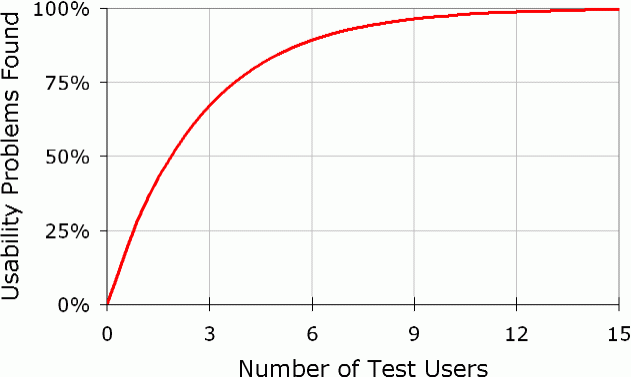
\includegraphics[width=\linewidth]{figures/fiveplot}
	\caption{A plot illustrating the usability problems found with the users.\cite{5users}}
	\label{fig:5plot}
\end{figure}

\subsubsection{Order of Evaluation}

As the order of prototypes with different solution ideas presented in evaluation could influence the user, as they tend to learn. Therefore, we change the order for different segments of users, which could lead to a qualitative result. For instance, let us say there are two prototypes named A and B. Half of users, i.e., three in our case will have prototype A tested first and another half, i.e., two users will test B first. This re-ordering helps to avoid recency bias cognitive error and priming effect as mentioned in Chapter \ref{ch:limitations_report}. \\

\subsection{Affinity Notes}

We use affinity notes \cite{affinity} for extracting the verbal data recorded during user study sessions. It is the most commonly used technique in the field of human-computer interaction research. Each affinity note is a piece of paper, where we write factual statements, observations or quotations. Additionally, in our scenario, we also mention timestamp, user id, research question id and prototype design id. Once, we finish preparing affinity notes for all users in a design cycle; we place them everything on a wall called Affinity Wall. Next, we sort the affinity notes papers into proper clusters such as solution ideas, research question. This clustering helps to analyse the data and understand the results, i.e., formative feedback or qualitative data. \\


\subsection{Usability Inspection Methods}

There are many usability inspection methods \cite{nielsen1994usability} like Heuristic evaluation, Heuristic estimation, Cognitive walkthrough, Pluralistic walkthrough, Feature inspection, Consistency inspection, Standards inspection and Formal usability inspection. Out of which, we test the usability aspect of the prototypes with ‘Cognitive walkthrough’. \\ \\

\subsubsection{Cognitive Walkthrough}

In a cognitive walkthrough, we ask users to perform tasks which has pre-defined steps. An example of a task could be finding a common bug reported by available tools. For each step, there are questions examined to determine usability. Blackmon et al. in their paper \cite{blackmon2002cognitive} mentions four questions which are significant to analyse while performing Cognitive Walkthrough for the Web. They are; \\

\begin{enumerate}
\item Will the user be able to try and attain the right conclusion?
\item Will the user be able to notice the presented right action on UI?
\item Will the user be able to associate the right action with the outcome they expect to accomplish?
\item If the user makes right action; will he be able to see as progress made towards their intended conclusion?
\end{enumerate}

These questions are also quite applicable in our context, and so, we assess these questions for each step. The designed elements on the user interface predetermines in order to solve a research question. So, the steps vary for each design. This approach gives qualitative feedback from a user as they are a mostly open-ended scenario to discuss primarily, for questions which users answers as ‘No’ would lead to having their suggestions/feedback. \\ \\

Overall, cognitive walkthrough helps to identify the usability problems in detail as possible, which is a qualitative analysis. Further, when we need to evaluate two best solution ideas against each other, then a polling method with a simple choice of solution idea and a usability rating are considered. It is merely to estimate which is more accepted by users with a parameter of the majority where more number of users/evaluators could determine the stronger validity of voting, which is a quantitative analysis. \\ \\

\clearpage

\subsubsection{Likert Scale}

In the process of testing the opinions of a person on a particular topic or question in specific, it is better to test how strongly they agree or not rather than stating agree or disagree. For this kind of evaluation, we use a scale called a Likert scale. \cite{likert} Mr Rensis Likert, who is American Social Psychologist, has created it and so named after him. \\ \\

We use Likert scales for closed-ended questions. It helps to get a detailed analysis of the designs proposed in this thesis whether how likely they are usable in terms of user perspective instead of answering binary questions of yes or no. Likert Scales are of two types, i.e., Uni Polar and Bi-Polar. \\ \\

Uni Polar Likert Scale shows one attribute let us say ‘strongly agree’ on one end and ‘I do not agree’ on the other end. Incase of Bi-Polar Likert Scale it shows ‘strongly agree’ on one side and ‘strongly disagree’ on the other side, and also there is a label in the middle which usually states ‘neither’. In this thesis work, we use the ‘Uni Polar Likert Scale’ with labels 0 and 10 on either end of a scale showing ‘not at all usable’ to ‘highly usable’. Not at all usable could be understood as the worst design or solution idea for an user scenario.\\ \\

\subsubsection{Metrics}

While testing the designs, we consider the following metrics — the evaluation results in quantitative feedback on solution ideas.

\begin{enumerate}
\item task success
\item perceived usability rating
\end{enumerate}

Task success determines whether the user can perform the given task based on success criteria respective to each task. The user provides the perceived usability rating in comparison on the scale of 0 to 10, 0 being low and 10 be higher with Uni Polar Likert Scale of attribute high usable on one end and not at all usable on other end. It determines how usable is a design in comparison to alternate design. 


\let\cleardoublepage\clearpage


